\documentclass{beamer}

\usetheme{Boadilla}
\usecolortheme{crane}
\usepackage{multicol}
\usepackage{graphicx}

\title{\textbf{Git Bootcamp}}
\subtitle{\textit{Computer Student Society}}
\author{Nate Dolny}
\date{}

\begin{document}

% title page 
\begin{frame}
	\titlepage
\end{frame}

% What is git?
\begin{frame}{What is Git?}
	\frametitle{\textbf{What is Git?}}
	\begin{itemize}
		\item One of the many popular version control systems available
	\end{itemize}

	\begin{center}
		
\includegraphics[width=0.2\textwidth]{img/Git-Logo.png} 
		\hspace{1cm}
		
\includegraphics[width=0.2\textwidth]{img/Mercurial_logo.png} 
		\hspace{1cm}
		
\includegraphics[width=0.2\textwidth]{img/Apache_Subversion_logo.png} 
		\hspace{1cm}
	\end{center}	

	\begin{itemize}
		\item Git is a tool used to manage code but can also be applied to any other type of document (\textbf{does not have to be code})
	\end{itemize}
	
	\begin{block}{\textbf{Version Control}}
		\textit{Records changes a person made to a document overtime. It can be used by one person or multiple people.}
	\end{block}
\end{frame}

\begin{frame}{Where did it come from?}
	\frametitle{\textbf{History of Git}}
	
	Started over a license dispute between Linus Torvalds and BitKeeper. Basically
BitKeeper, the source code management system for the Linux kernel and many other open source projects, revoked the Linux developer’s free license. Bitkeeper’s parent company did this because an open source developer, attempted to create an open-source version of the BitKeeper client without accepting its proprietary license.

	\begin{center}
		\includegraphics[width=0.3\textwidth]{img/BitKeeper_logo.png} 
		\hspace{1cm}
		\includegraphics[width=0.5\textwidth]{img/linux.jpeg} 
	\end{center}

\end{frame}

\begin{frame}
	\frametitle{\textbf{History of Git}}

\begin{itemize}
\item Git was built in about 5 days
\item Released in April 2005 by Linus Torvalds 
\end{itemize}

\vspace{0.5cm}
\textbf{Design goals of Git:}
 
\begin{itemize}
\item Speed 
\item Simple design 
\item Fully distributed 
\item Strong support for non linear development (branching)
\item Able to handle large projects such as the linux kernel 
\end{itemize}

\end{frame}


% Why do should you use Git?
\begin{frame}
	\frametitle{\textbf{Why you should use Git?}}
	
	\textbf{Organization:}
	\begin{itemize}
		\item Tracks changes on a document
		\item Allows for multiple users to work on the same document
	\end{itemize}

	\vspace{0.25cm}
	\textbf{Branching:}
	\begin{itemize}
		\item Allows for multiple branches to be created (more later)
	\end{itemize}

	\vspace{0.25cm}
	\textbf{Backups:}
	\begin{itemize}
		\item Acts as a backup when used remotely (\textbf{should not be your main backup})
	\end{itemize}

	\vspace{0.25cm}
	\textbf{Machine Agnostic:}
	\begin{itemize}
		\item Can be used on any operating system: Windows, Mac, GNU Linux
	\end{itemize}

\end{frame}


% When should you use Git?
\begin{frame} 
	\frametitle{\textbf{When should you use Git?}}
	\begin{itemize}
		\item \textbf{ALWAYS!!}
		\item Git is your best friend when it comes to any project big or small  
	\end{itemize}
\end{frame}

% level One
\begin{frame}
	\begin{figure}[h]
	\centering
	\includegraphics[width=0.8\textwidth]{img/levelone.png} 
	\end{figure}
\end{frame}

% Setting up Git
\begin{frame}
	\frametitle{\textbf{Setting up Git}}

	\textbf{Create a Profile}
	\vspace{0.5cm}

	\textit{Set Profile Name}
	\begin{itemize}
		\item git config --global user.name "Peter Parker"
	\end{itemize}

	\textit{Set Profile Email}
	\begin{itemize}
		\item git config --global user.name "Parker.P@midtown.net"
	\end{itemize}

	\textit{Set Default Editor}
	\begin{itemize}
		\item git config --global editor="vim"
	\end{itemize}

	\textit{View our configuration (Optional)}
	\begin{itemize}
		\item git config --global list
	\end{itemize}

	\begin{block}{\textbf{PRO TIP}}
		\textit{Git allows for multiple profiles, so you could have a personal and 
		school profile.}
	\end{block}
\end{frame}

% Command-line Text Editors 
\begin{frame}
	\frametitle{\textbf{Command-line Text Editors}}
	
	\begin{itemize}
		\item A text editor that can run directly in a terminal without a graphical user interface
	\end{itemize}

	\begin{figure}[h]
			\centering
			
\includegraphics[width=0.2\textwidth]{img/Vim_logo.png} 
			\hspace{0.5cm}
			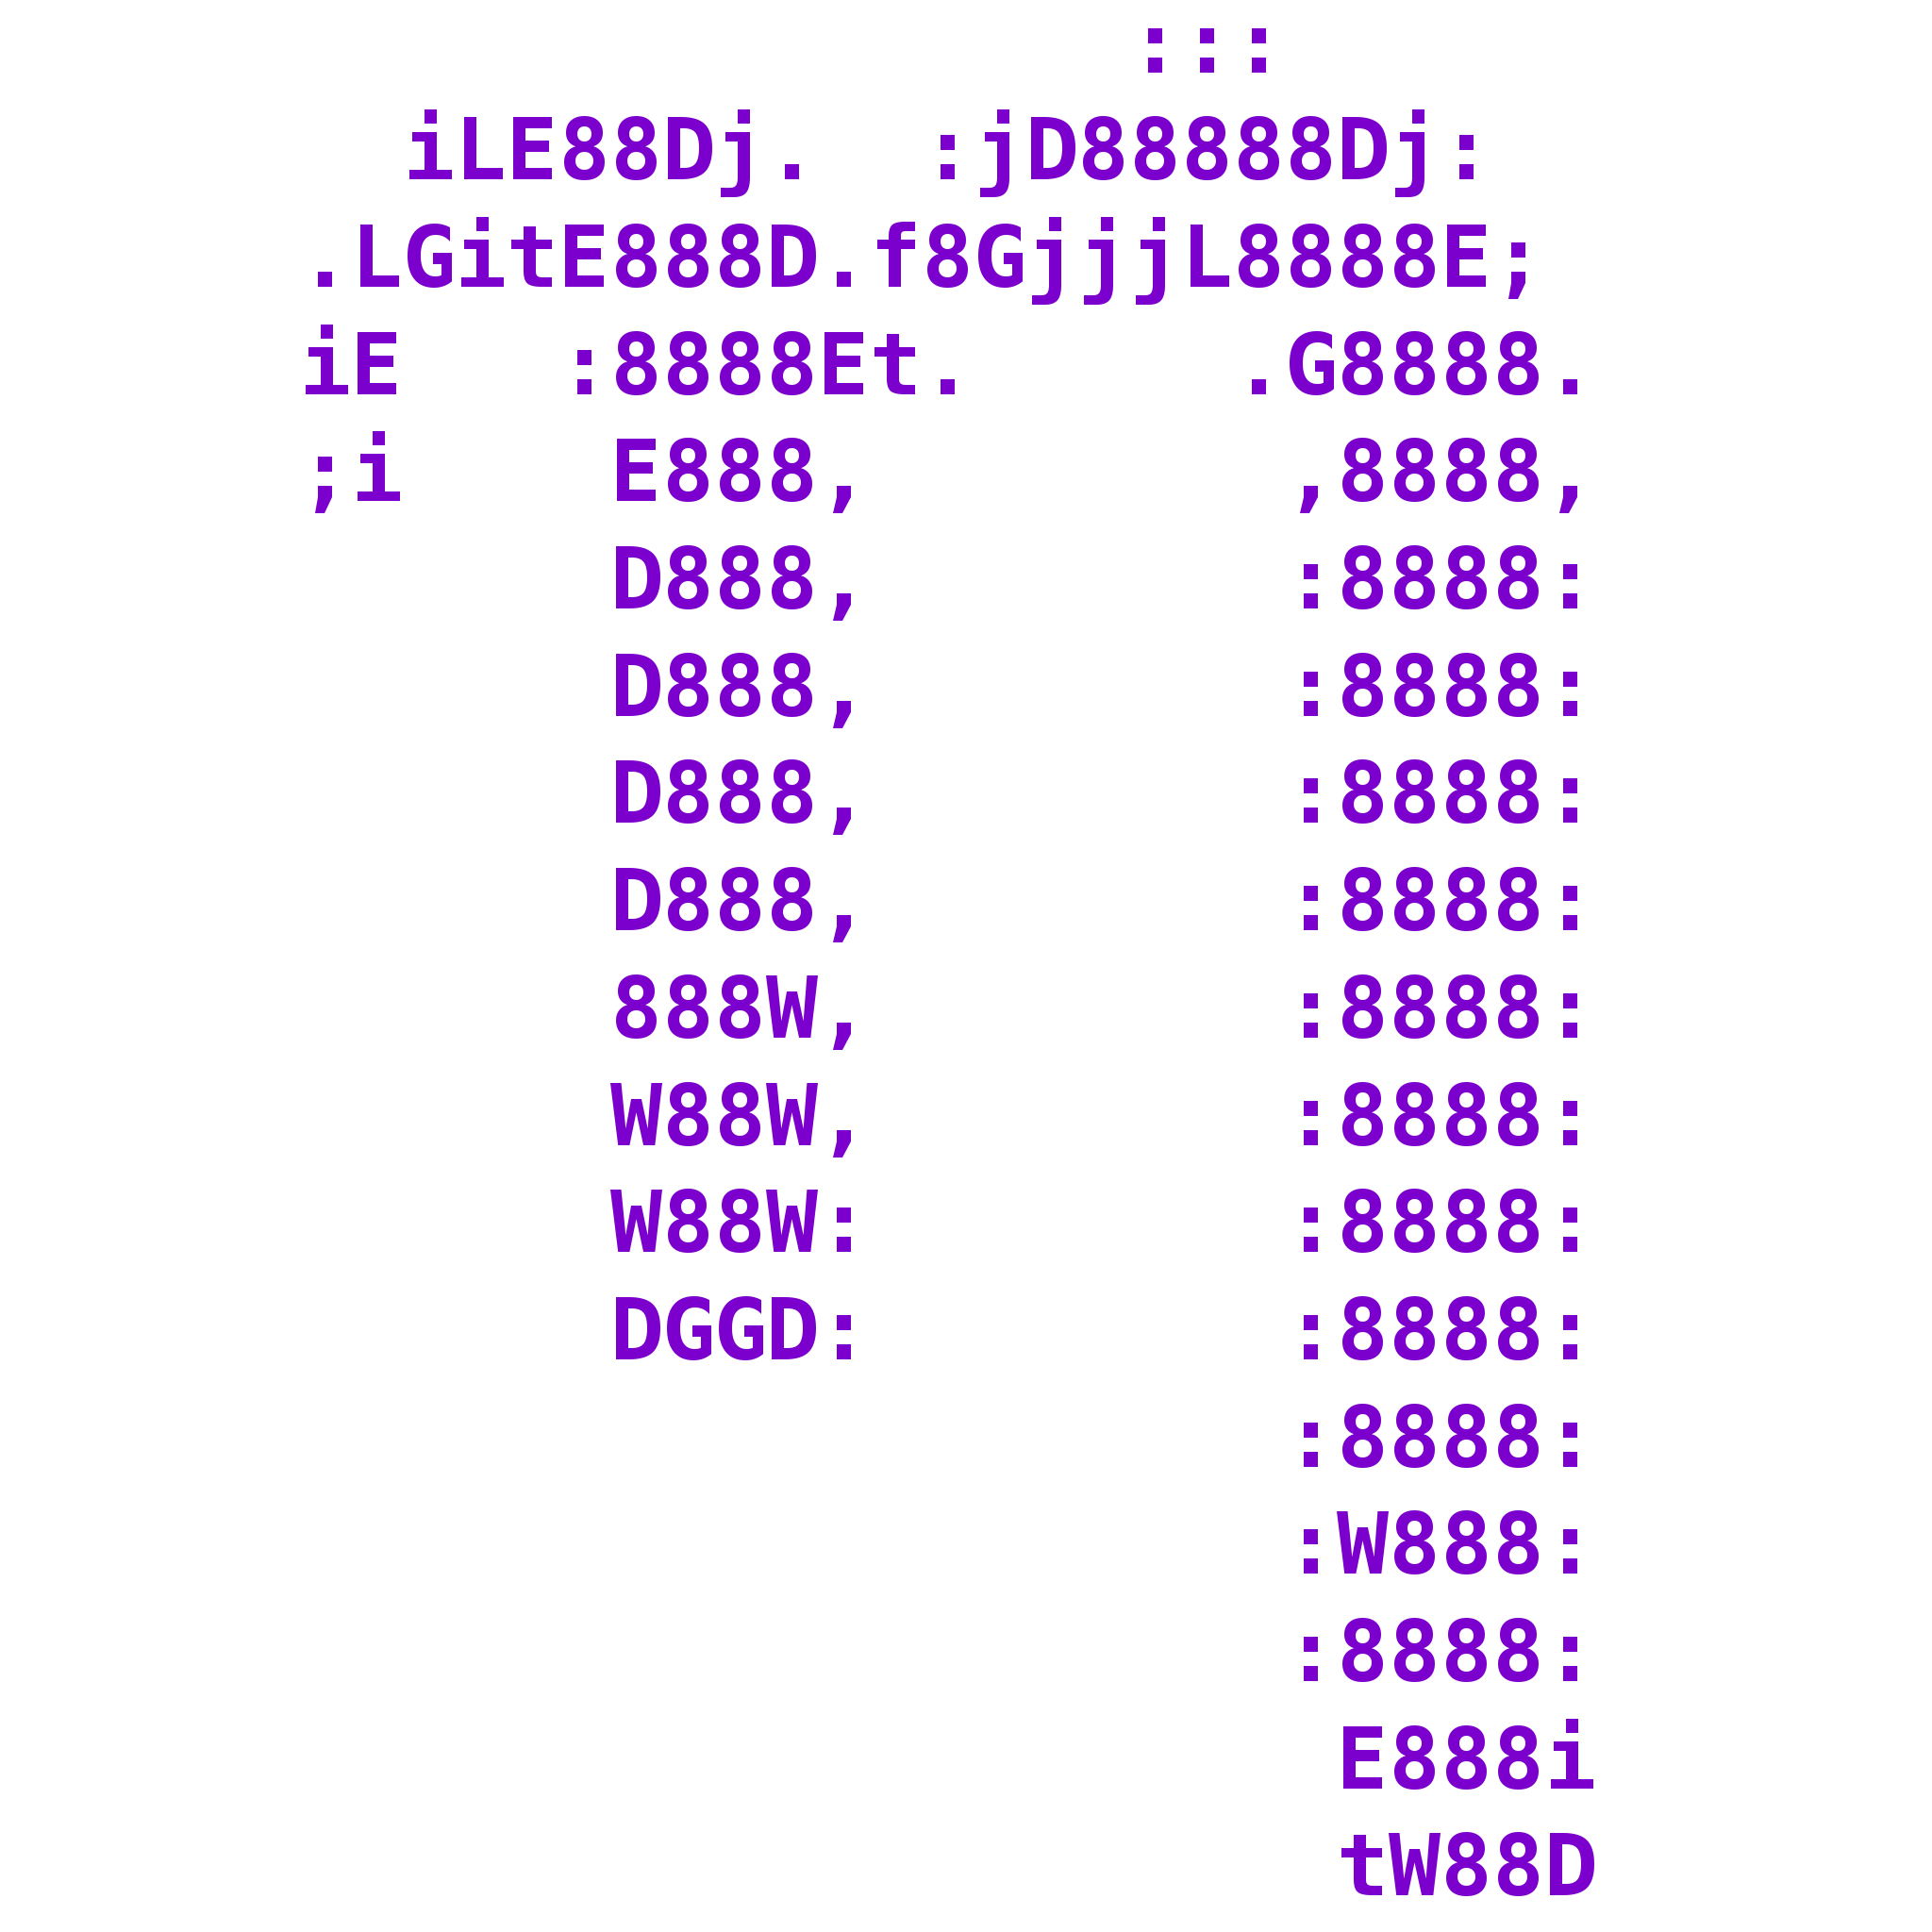
\includegraphics[width=0.2\textwidth]{img/nano_logo.png} 
			\hspace{0.5cm}
			
\includegraphics[width=0.2\textwidth]{img/Emacs_logo.png} 
	\end{figure}
\end{frame}

% Nano Text Editor 
\begin{frame}
	\frametitle{\textbf{GNU Nano Text Editor}}
		
	\begin{multicols}{2}
		\begin{figure}[h]
			\centering
			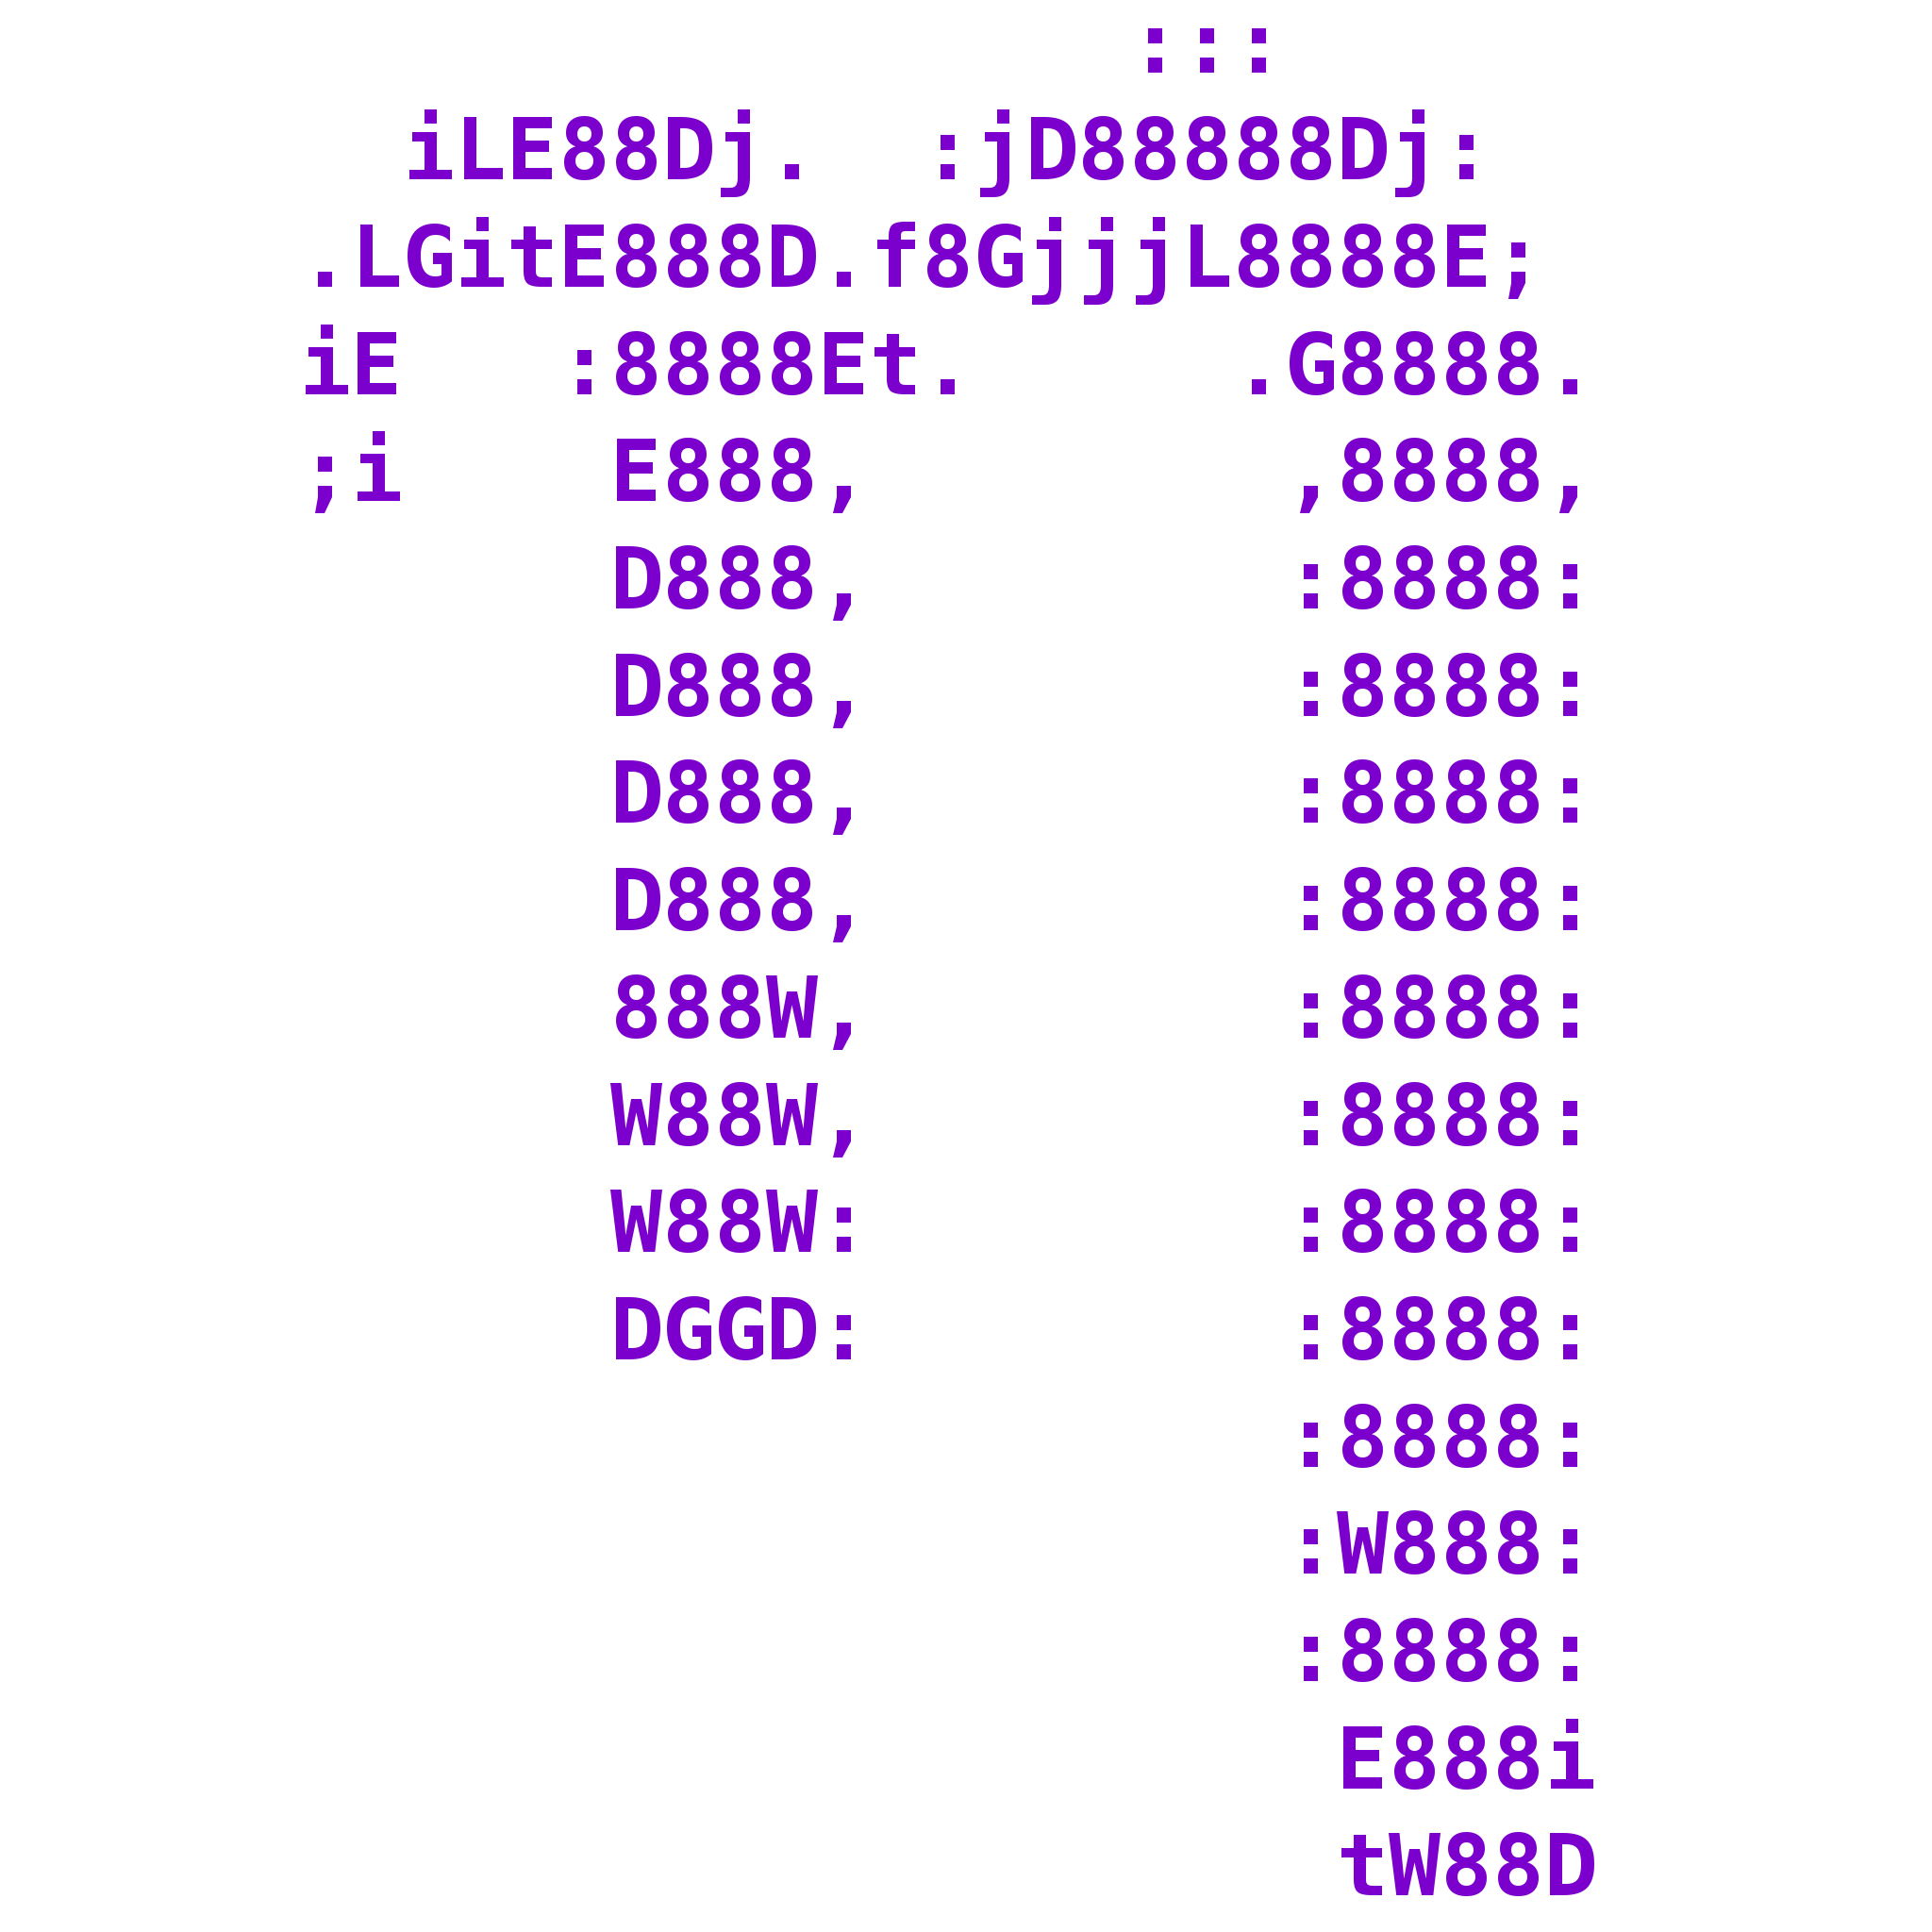
\includegraphics[width=0.2\textwidth]{img/nano_logo.png} 
		\end{figure}

		\begin{itemize}
			\item Released in November 18, 1999
			\item User-friendly and easy to learn 
			\item Developed and maintained by volunteers
		\end{itemize}

		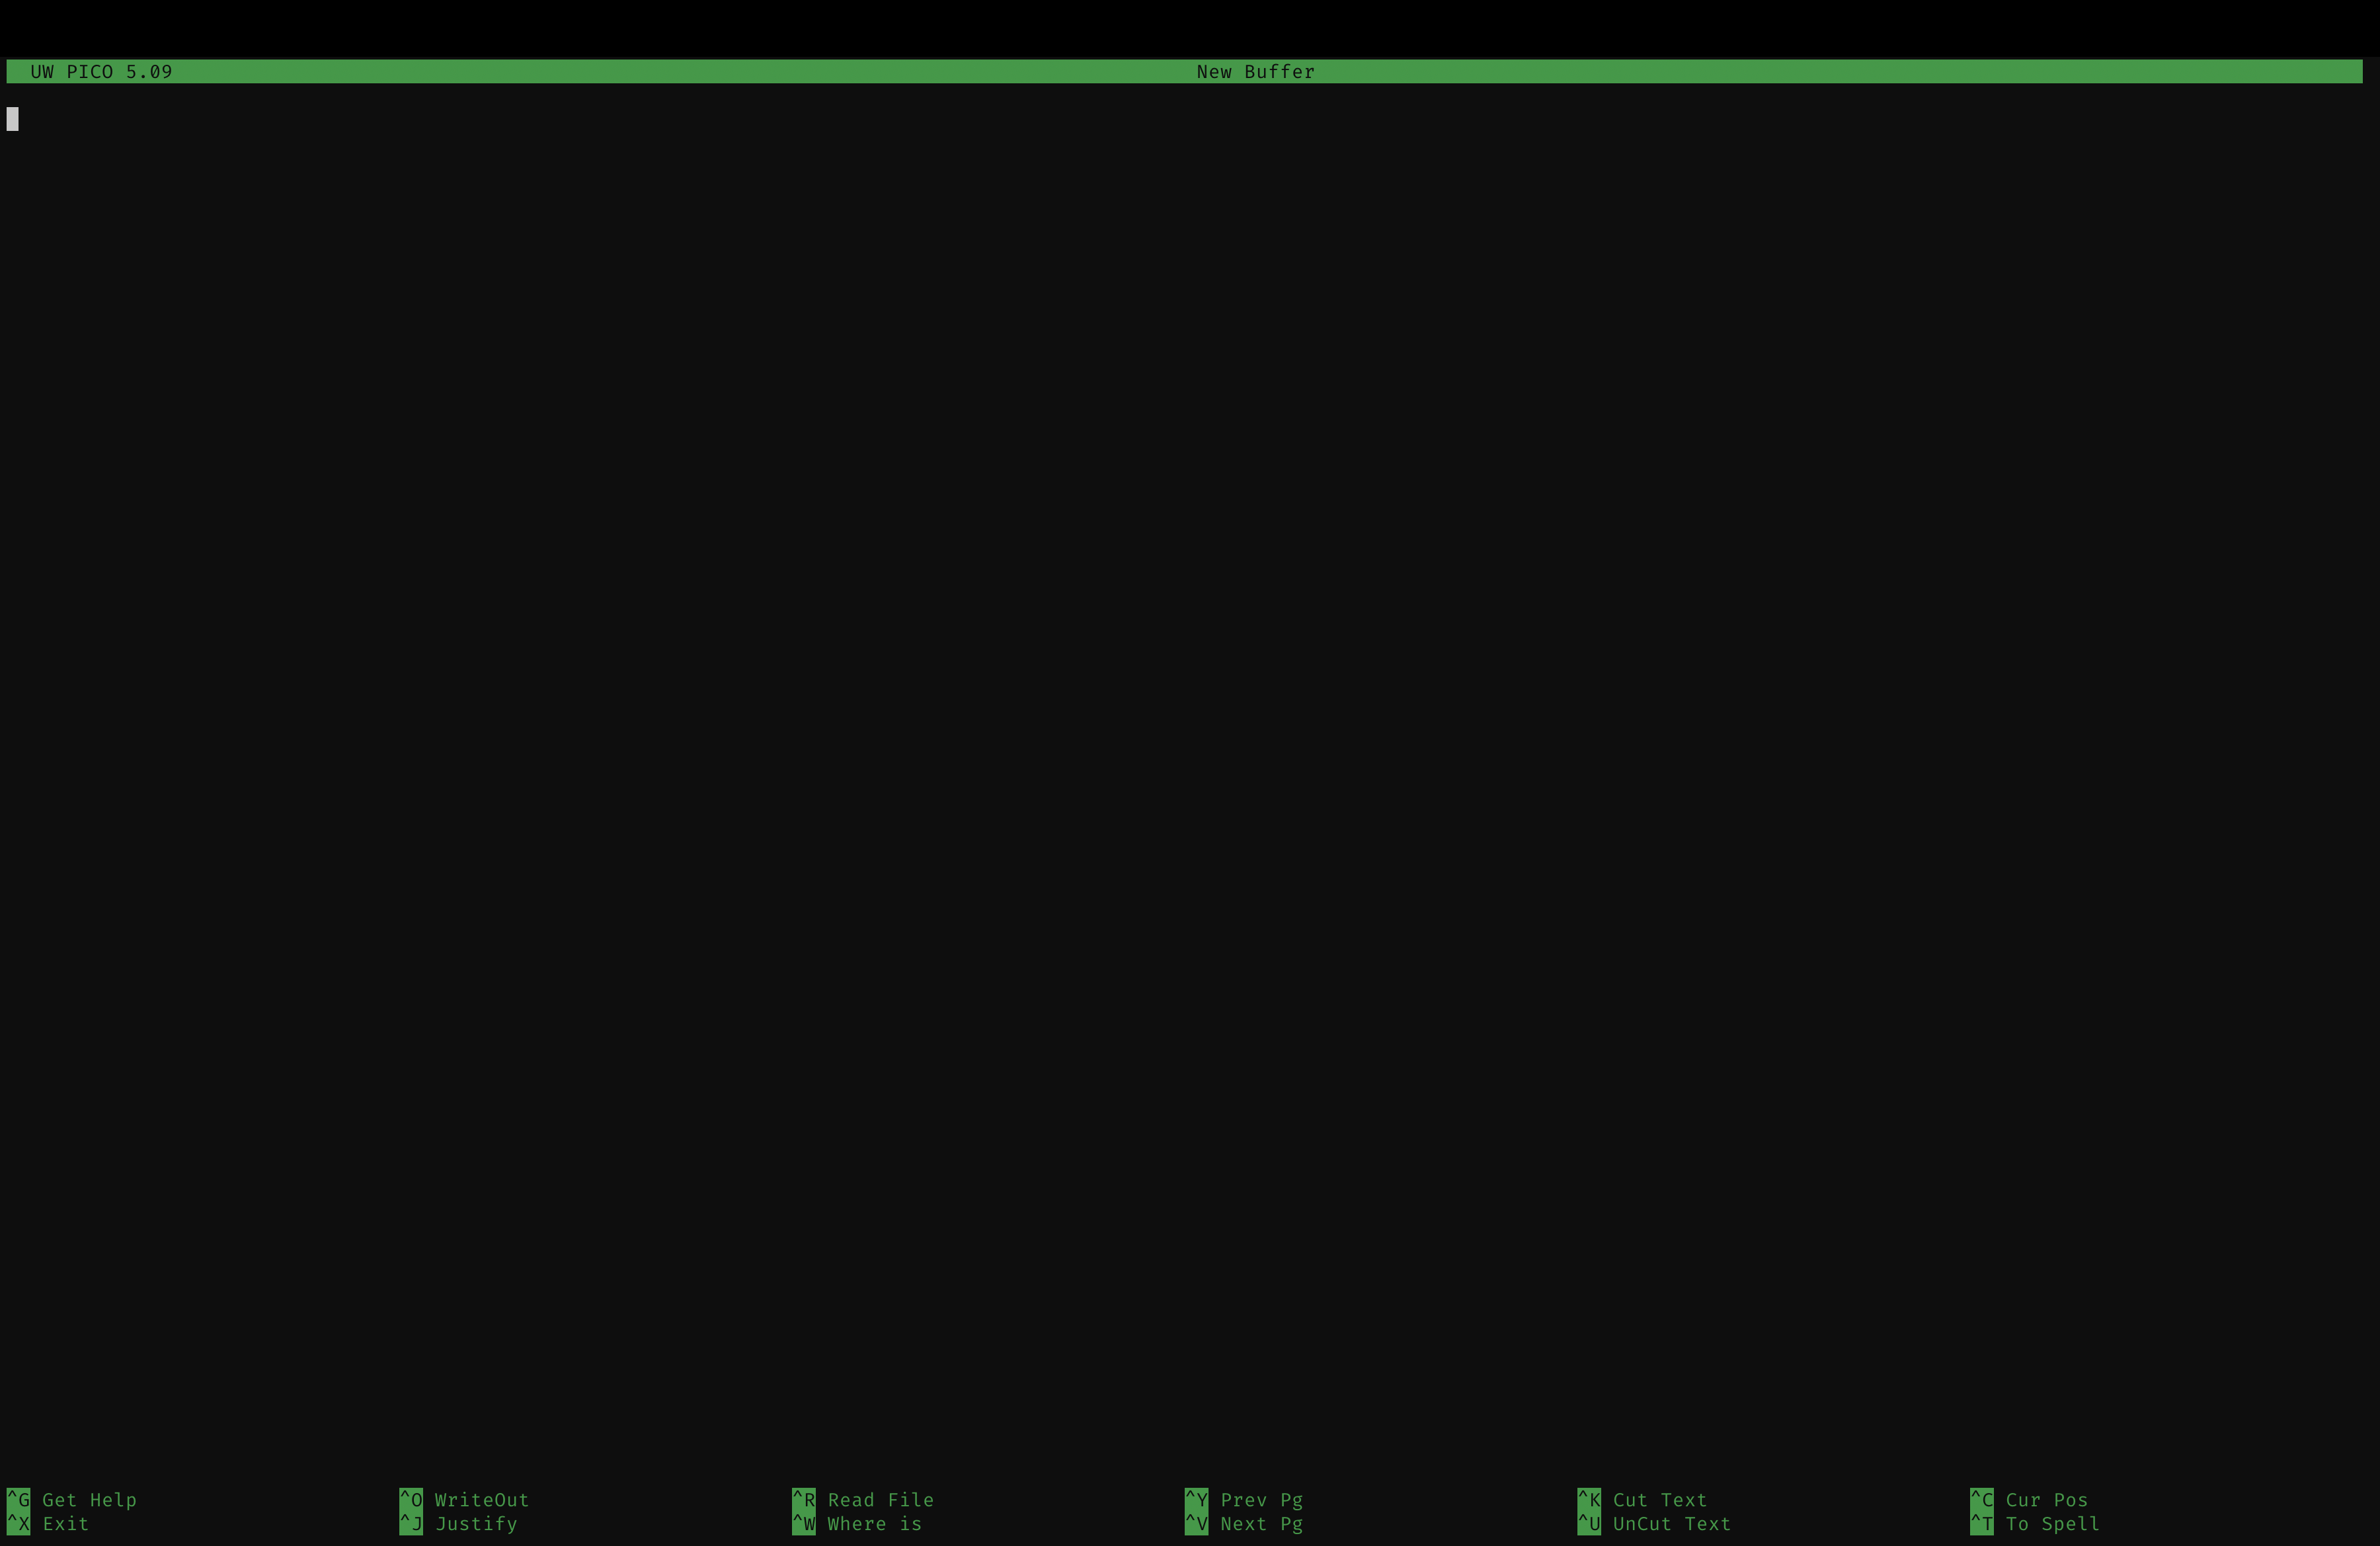
\includegraphics[width=0.5\textwidth]{img/nano.png} 
	\end{multicols}

\end{frame}

% Vim Text Editor 
\begin{frame}
	\frametitle{\textbf{Vim Text Editor}}
		
	\begin{multicols}{2}
		\begin{figure}[h]
			\centering
			
\includegraphics[width=0.2\textwidth]{img/Vim_logo.png} 
		\end{figure}

		\begin{itemize}
			\item Released in November 2, 1991
			\item Modal editor 
			\item Highly customizable, many plugins available 
		\end{itemize}

		\includegraphics[width=0.5\textwidth]{img/Vim.png} 
	\end{multicols}
\end{frame}

% Emacs Text Editor 
\begin{frame}
	\frametitle{\textbf{Emacs Text Editor}}
		
	\begin{multicols}{2}
		\begin{figure}[h]
			\centering
			
\includegraphics[width=0.2\textwidth]{img/Emacs_logo.png} 
		\end{figure}

		\begin{itemize}
			\item Released in March 20, 1985
			\item Created by GNU Project founder Richard Stallman
			\item Highly customizable
			\item Many modes for different purposes such as browsing the web
		\end{itemize}

		\includegraphics[width=0.5\textwidth]{img/Emacs.png} 
	\end{multicols}
\end{frame}

% What makes a good commit
\begin{frame}
	\frametitle{\textbf{What makes a good commit?}}
	
	\begin{itemize}
		\item Detailed messages that someone can read that informs others about the
changes you made to a document. 
	\end{itemize}

	\begin{figure}[h]	
		\centering
		
\includegraphics[width=0.5\textwidth]{img/minorchanges.jpeg} 
	\end{figure}

\end{frame}

\begin{frame} 
	\frametitle{\textbf{What makes a good commit?}}
	
	\textbf{A better approach to making commits} 
	\vspace{0.5cm}
	
	\begin{itemize}
		\item \textit{Title:} Add a topic
		\vspace{0.5cm}
		\item \textit{Changes:} Add details about changes made to file(s)
		\vspace{0.5cm}
		\item \textit{State:} Add a brief summary of the state of program or feature
		\vspace{0.5cm}
		\item \textit{TODO:} Make notes about things to fix
	\end{itemize}	

	\begin{block}{\textbf{PRO TIP}}
		Pretend you are sending an email to your friends, group mates, or professor
		informing them of the changes you made to the document.
	\end{block}

\end{frame} 

% Making a Commit 
\begin{frame}
	\frametitle{\textbf{Making a Commit}}

	\textbf{Step 1.} \textit{Add a document to staging}
	\begin{itemize}
		\item git add \(\prec document \succ\)
	\end{itemize}

	
	\vspace{0.5cm}

	\textbf{Step 2.} \textit{View documents that have been staged (Optional)}
	\begin{itemize}
		\item git status
	\end{itemize}

	
	\vspace{0.5cm}

	\textbf{Step 3.} \textit{Remove a document from staging (Optional)}
	\begin{itemize}
		\item git reset \(\prec document \succ\)
	\end{itemize}


	\vspace{0.5cm}

	\textbf{Step 4.} \textit{Record changes to repository}
	\begin{itemize}
		\item git commit
	\end{itemize}


	\vspace{0.5cm}

	\textbf{Step 5.} \textit{Upload changes to remote repository}
	\begin{itemize}
		\item git push 
	\end{itemize}
\end{frame}

% play time
\begin{frame}
	\begin{figure}[h]
	\centering
	\includegraphics[width=0.8\textwidth]{img/playtime.png} 
	\end{figure}
\end{frame}

% break time 
\begin{frame}
	\begin{figure}[h]
	\centering
	\includegraphics[width=0.8\textwidth]{img/breaktime2.png} 
	\end{figure}
\end{frame}

% level two 
\begin{frame}
	\begin{figure}[h]
	\centering
	\includegraphics[width=0.8\textwidth]{img/leveltwo.png} 
	\end{figure}
\end{frame}

% Remote version control platforms 
\begin{frame}
	\frametitle{\textbf{Remote Version Control Platforms}}

	\begin{itemize}
		\item Allows you to store code some place other than your local machine
		\item Allows for multiple people to collaborate on a project 
	\end{itemize}

	\begin{figure}[h]
		\begin{flushleft}
		
\includegraphics[width=0.5\textwidth]{img/GitHub_Logo.png} 
		\end{flushleft}
		\centering
		
\includegraphics[width=0.5\textwidth]{img/GitLab_logo.png} 
		\begin{flushright}
		
\includegraphics[width=0.5\textwidth]{img/Bitbucket_Logo.png} 
		\end{flushright}
	\end{figure}

\end{frame}

% GitHub 
\begin{frame}
	\frametitle{\textbf{GitHub}}
		
	\begin{multicols}{2}
		\begin{figure}[h]
			\centering
			\includegraphics[width=0.3\textwidth]{img/GitHub_logo.png} 
		\end{figure}

		\begin{itemize}
			\item Released in April 2008 
			\item Microsoft acquired Github in 2012 
			\item Over 100 million users
			\item Hosts millions of open source projects
		\end{itemize}

		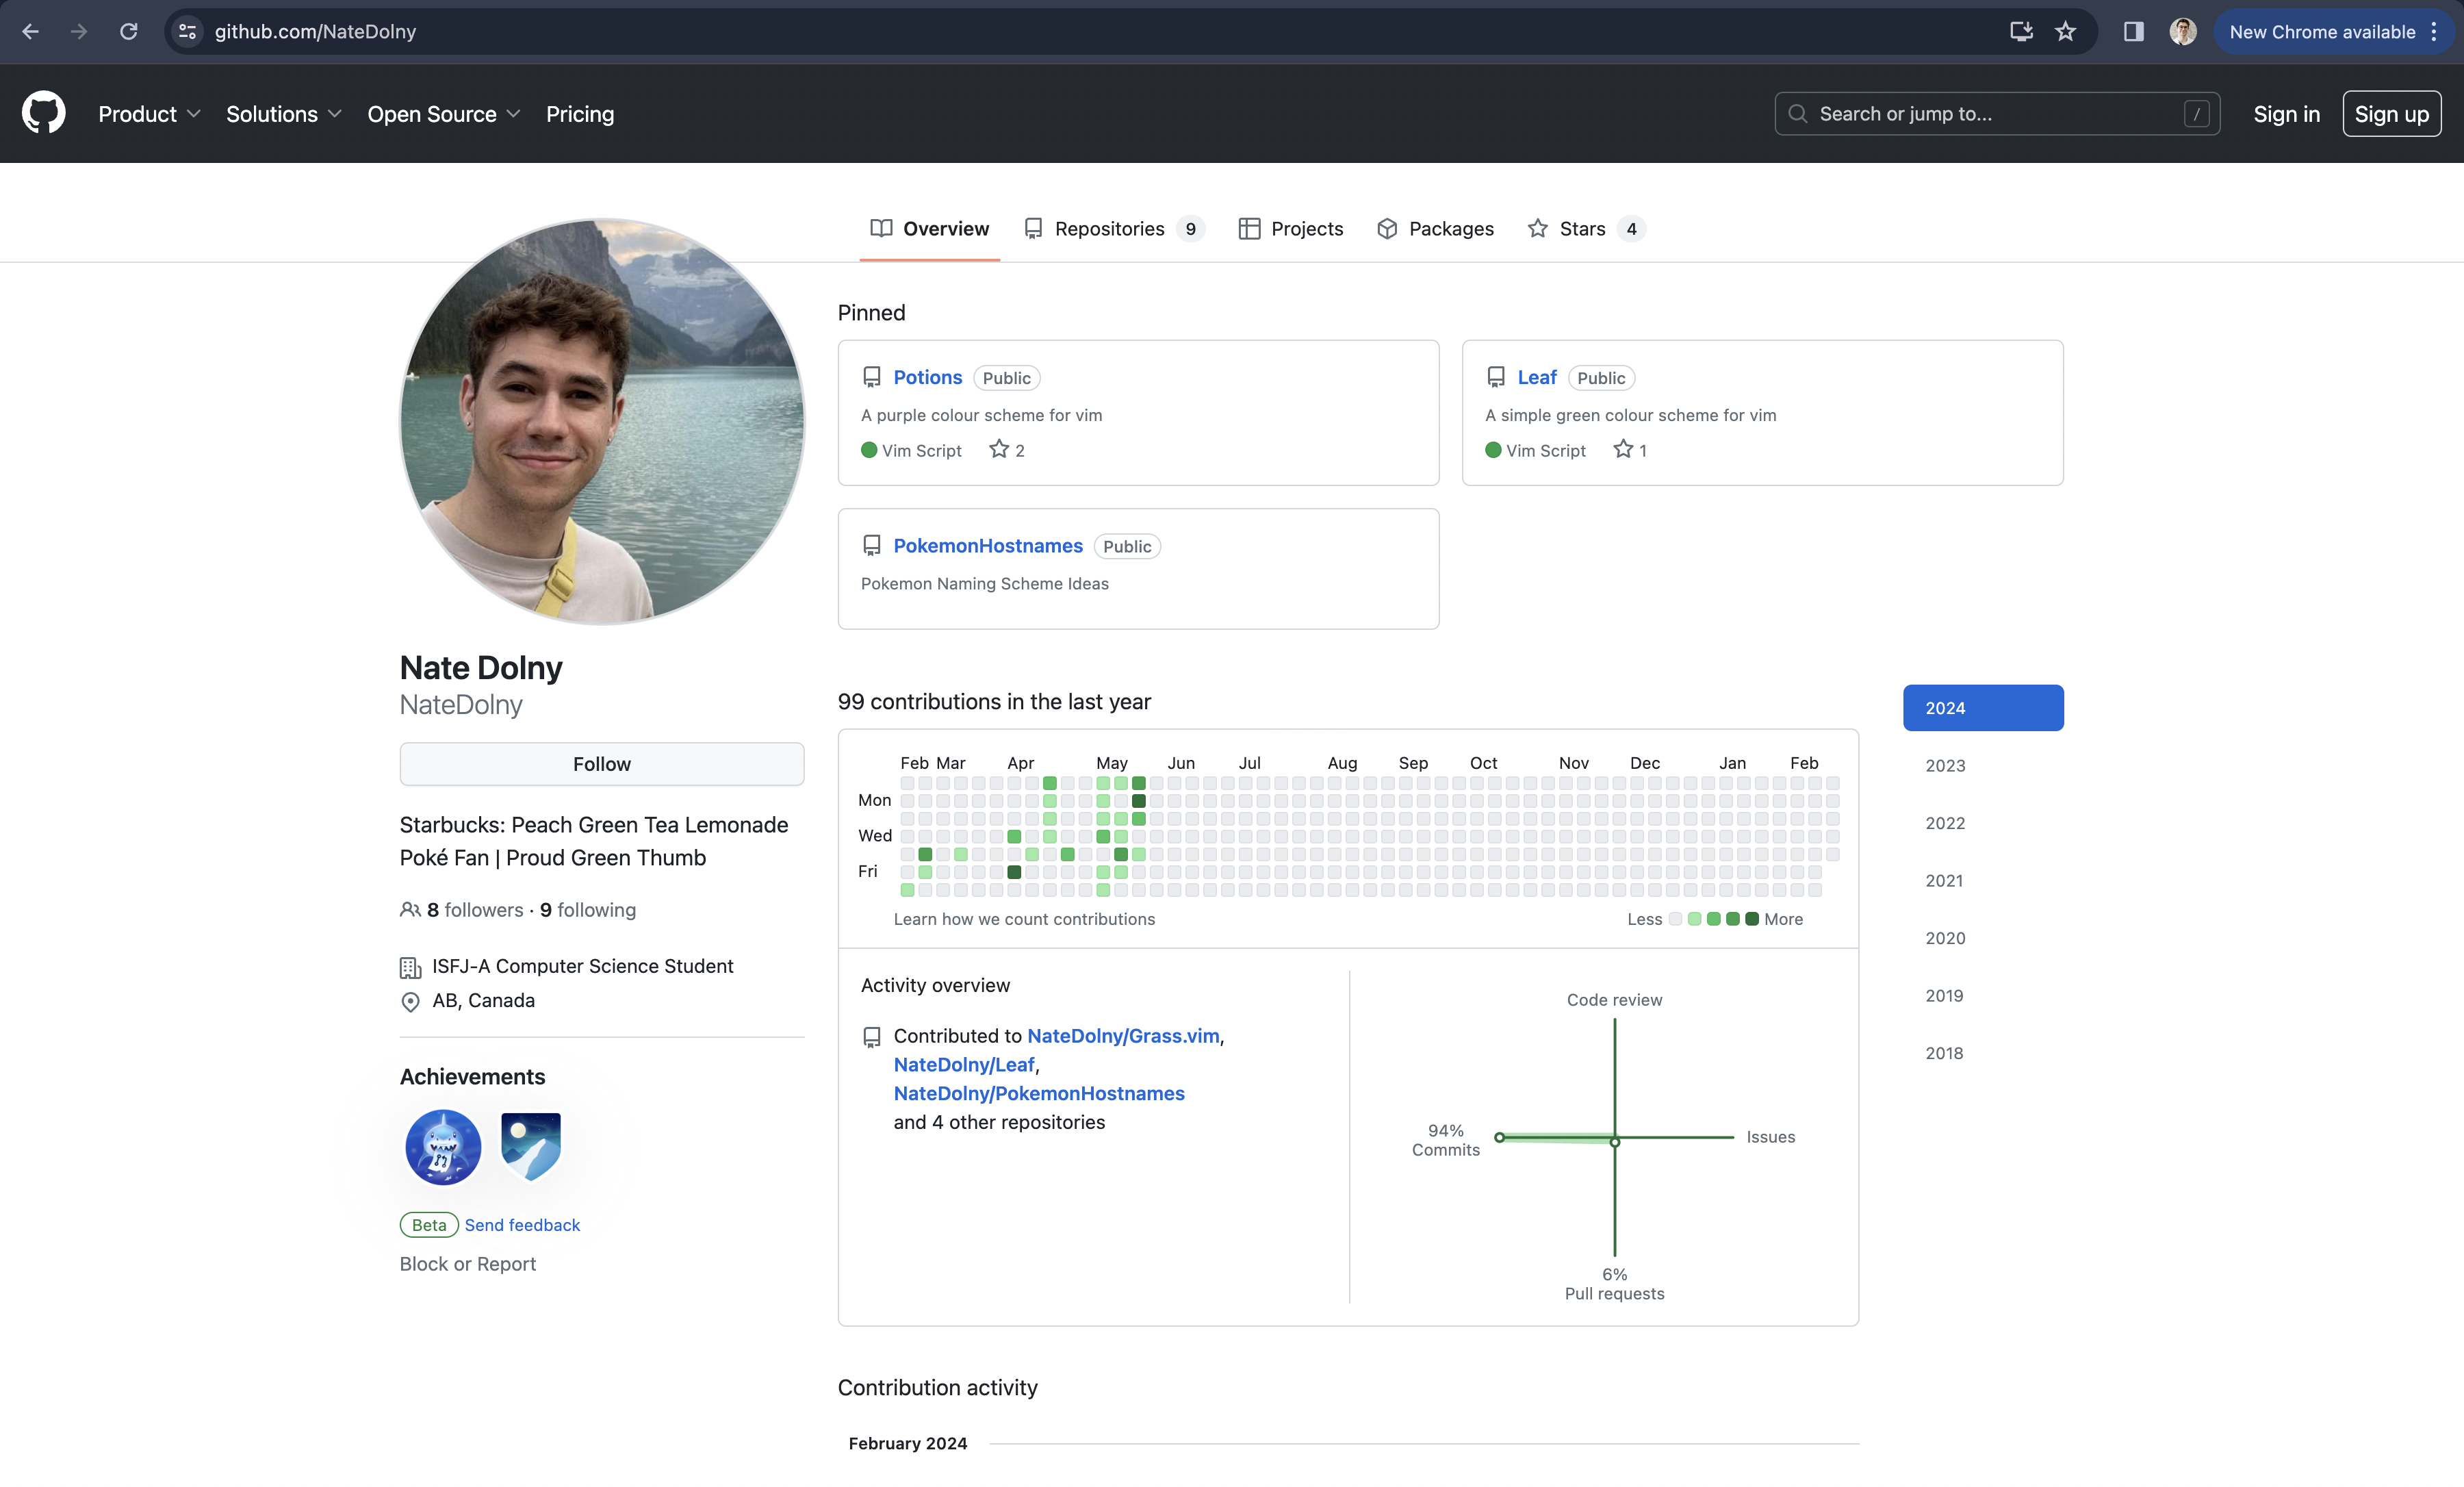
\includegraphics[width=0.5\textwidth]{img/github_ui.png} 
	\end{multicols}
\end{frame}

% Gitlab
\begin{frame}
	\frametitle{\textbf{GitLab}}
		
	\begin{multicols}{2}
		\begin{figure}[h]
			\centering
			
\includegraphics[width=0.3\textwidth]{img/GitLab_logo.png} 
		\end{figure}

		\begin{itemize}
			\item Released in 2011
			\item Over 30 million users
			\item More secure than GitHub
			\item Focuses on collaboration, efficiency, and automation 
			\item Only platform that self-hosting is free 
		\end{itemize}

		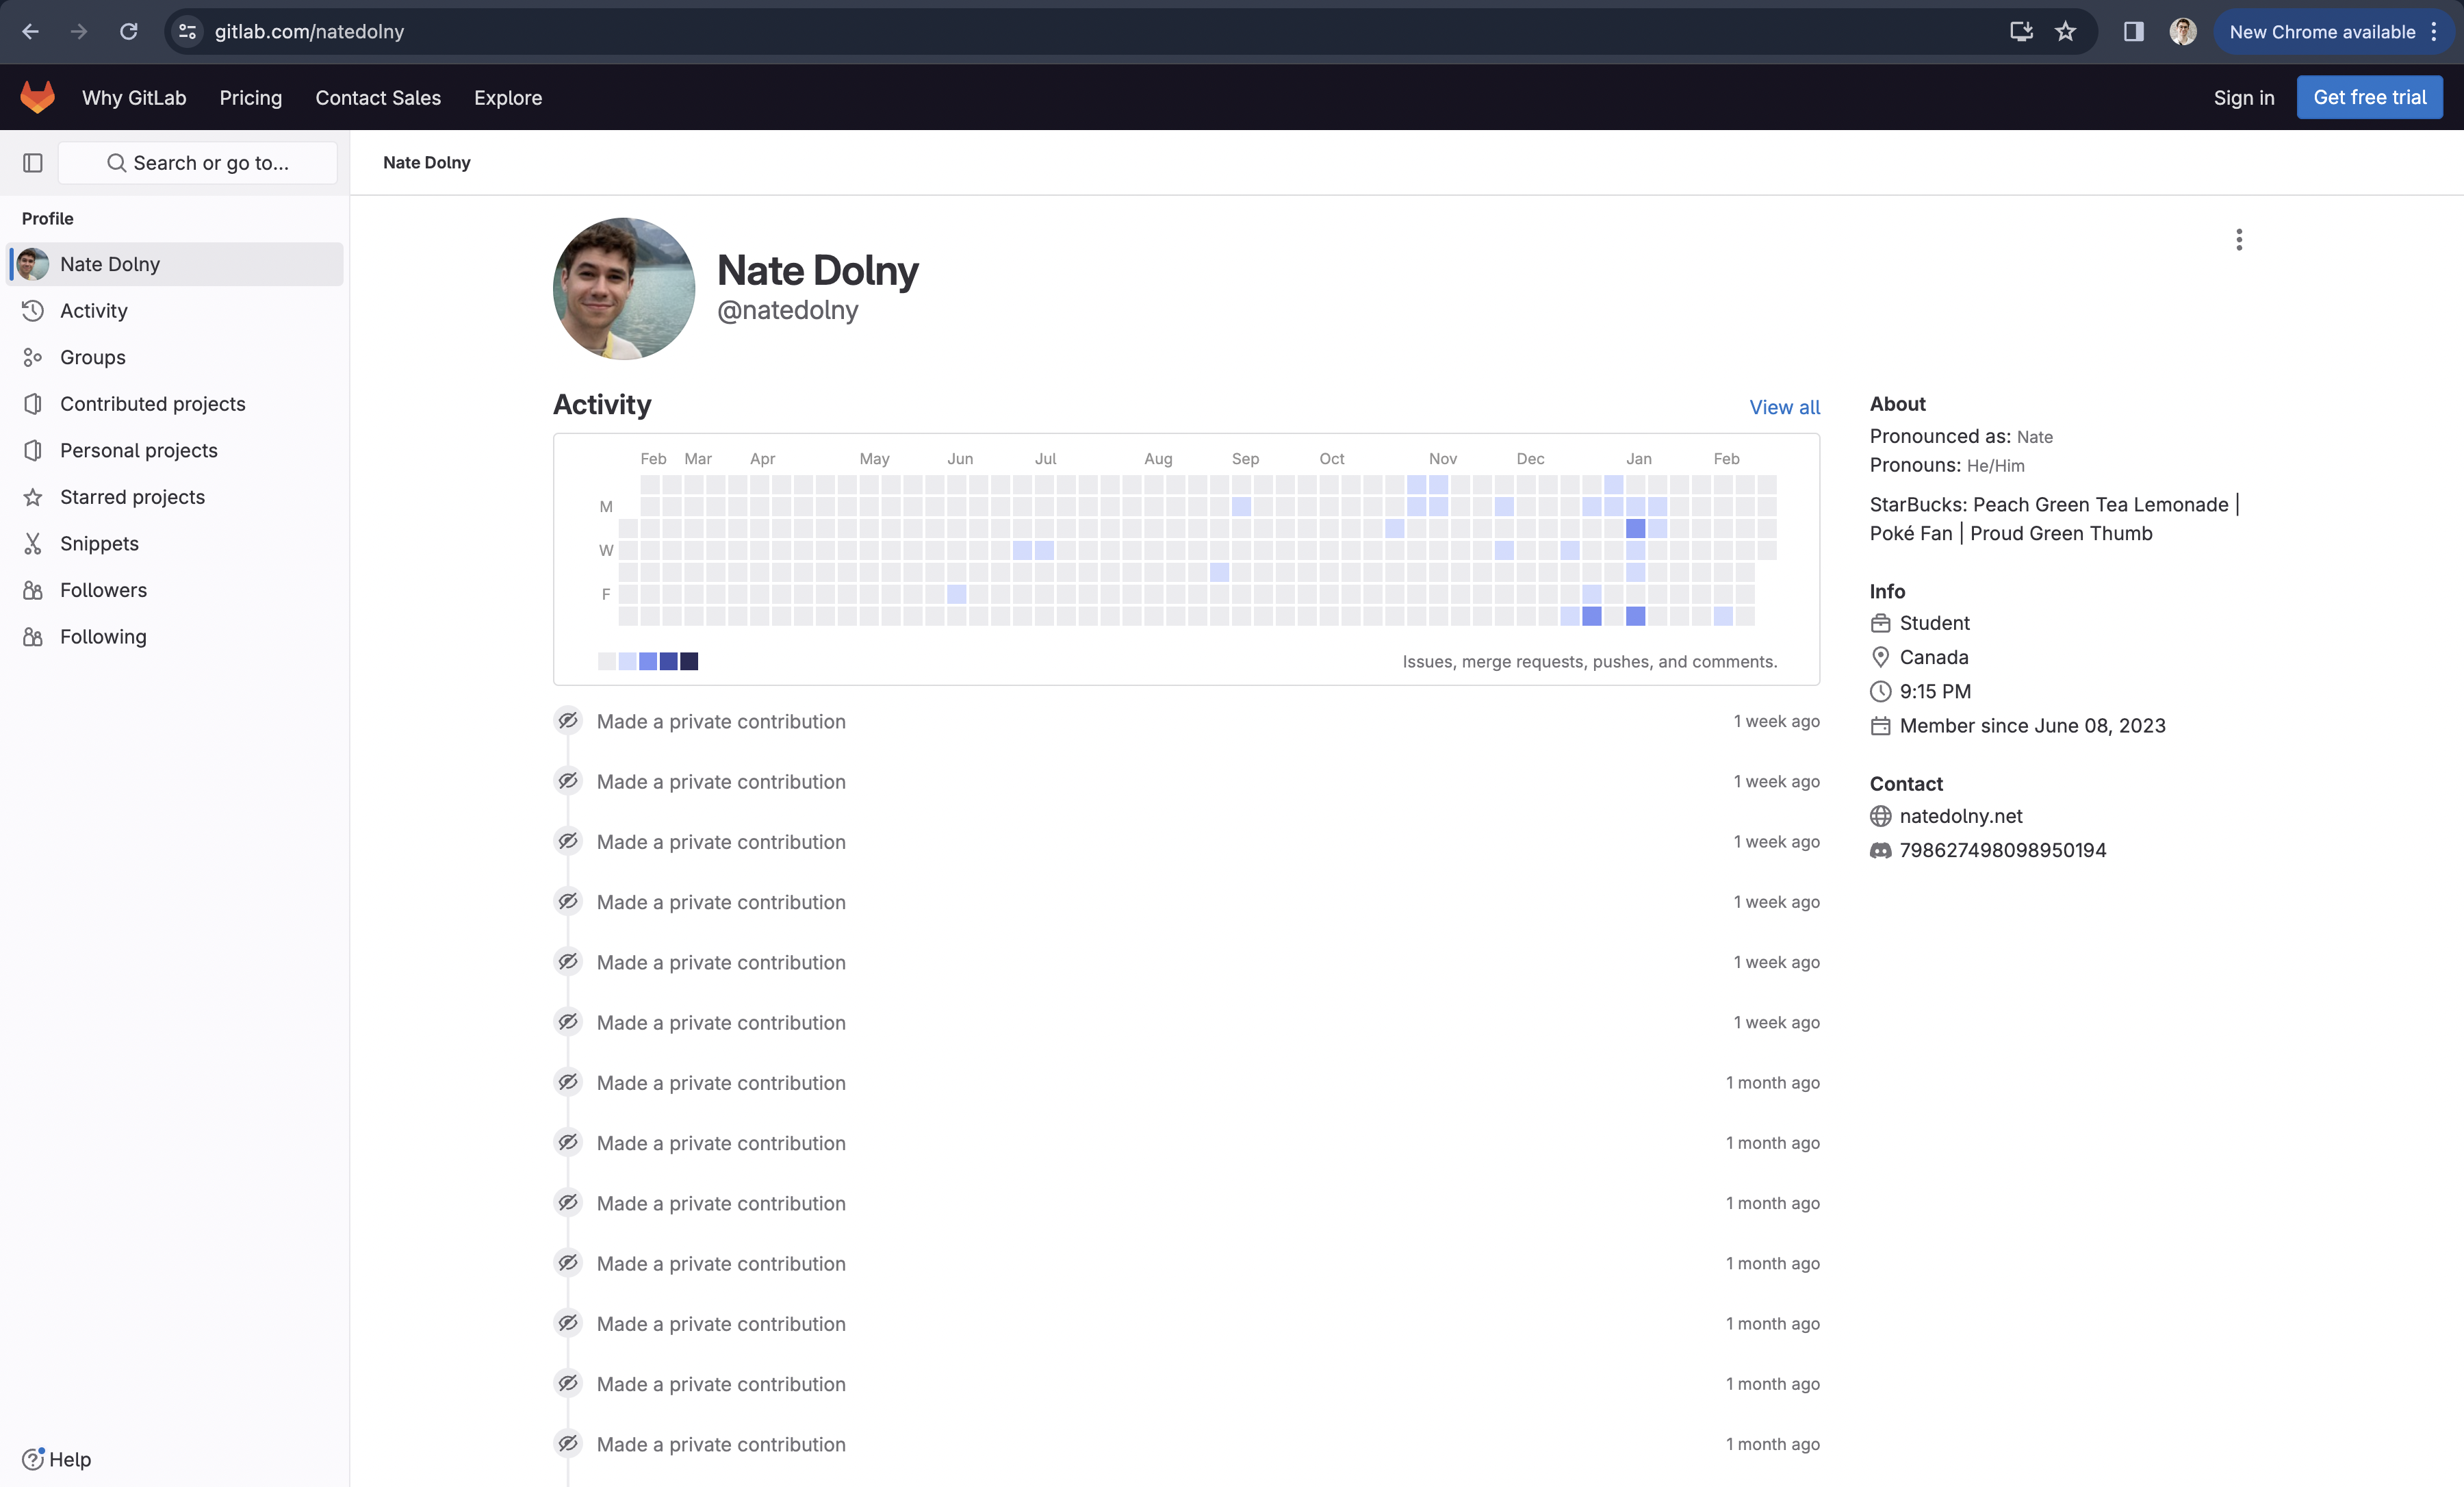
\includegraphics[width=0.5\textwidth]{img/gitlab_ui.png} 
	\end{multicols}
\end{frame}

% Intro to OpenSSH Suite
\begin{frame}
	\frametitle{\textbf{Introduction to OpenSSH Suite}}

	\begin{multicols}{2}
		\begin{figure}[h]
			\begin{flushleft}
			
\includegraphics[width=0.5\textwidth]{img/openssh.png}
			\end{flushleft}
		\end{figure}
		
		\begin{itemize}
			\item Encrypts all traffic to eliminate eavesdropping, connection hijacking, and other attacks.

			\vspace{0.2cm}
			\item ssh-keygen: Generates, manages, and converts authentication keys for ssh
			\item ssh-add: Adds private keys to the authentication agent
			\item ssh-scp: copies files between hosts on a network 
		\end{itemize}

		\begin{figure}[h]
			\begin{flushright}
			
\includegraphics[width=0.5\textwidth]{img/securityMeme.jpeg}
			\end{flushright}
		\end{figure}
	\end{multicols}
\end{frame}

% Create an SSH Key
\begin{frame}
	\frametitle{\textbf{Generate an SSH Key}}
	
	\textbf{Generate an SSH-Key}
	\begin{itemize}
		\item ssh-keygen -t ed25519 -C "Parker.P@midtown.net" 
	\end{itemize}
	\vspace{0.5cm}

	\textbf{You'll then be given a choice}
	"Enter a file which to save the key (/home/You/.ssh/id\_ALGORITHM):"	
	
	\vspace{0.5cm}
	\textbf{Option 1.} \textit{Name the key}
	\begin{itemize}
		\item Enter your chosen key name and press enter
	\end{itemize}

	\textbf{Option 2.} \textit{Press enter}
	\begin{itemize}
		\item Should only choose this option if you will only ever have one key
	\end{itemize}

	\begin{block}{}
		\textbf{Congrats you have created your first SSH Key!!}
	\end{block}

\end{frame}


% adding an ssh key to ssh agent 
\begin{frame}
	\frametitle{\textbf{Adding an SSH Key to the SSH-Agent}}

	\textbf{Step 1.} \textit{Start ssh-agent in the background}
	\begin{itemize}
		\item eval "\$(ssh-agent -s)"
	\end{itemize}

	\vspace{0.5cm}
	\textbf{Step 2.} \textit{Add your ssh key to the ssh-agent}
	\begin{itemize}
		\item ssh-add /.ssh/\(\prec yourKeyName \succ\)
	\end{itemize}

	\vspace{0.5cm}
	\textit{If you didn't name your key use this instead}
	\begin{itemize}
		\item ssh-add /.ssh/id\_ed25519 
	\end{itemize}
\end{frame}

% login into gitlab 
\begin{frame}
	\frametitle{\textbf{Exploring GitLab}}

	\begin{multicols}{2}
	%\begin{figure}[h]
	%		\centering
	%		
\includegraphics[width=0.3\textwidth]{img/GitLab_logo.png} 
	%\end{figure}

	\textbf{Open Firefox or Google Chrome}
	\begin{itemize}
		\item https://git.cs.usask.ca/users/sign\_in
	\end{itemize}

	\vspace{0.5cm}	
	\textbf{Username}
	\begin{itemize}
		\item \textit{Your NSID example: abc123}
	\end{itemize}

	\vspace{0.2cm}
	\textbf{Password}
	\begin{itemize}
		\item \textit{Your Canvas Password}
	\end{itemize}

	\begin{figure}[h]
			
\includegraphics[width=0.5\textwidth]{img/homer.png} 
	\end{figure}
\end{multicols}
\end{frame}

% adding our key to gitlab 
\begin{frame}
	\frametitle{\textbf{Adding our key to GitLab}}

	\textbf{Step 1.}
	\begin{itemize}
		\item \textit{Click on edit profile}
	\end{itemize}

	\textbf{Step 2.}
	\begin{itemize}
		\item \textit{Click on SSH Keys}
	\end{itemize}

	\textbf{Step 3.}
	\begin{itemize}
		\item \textit{Click on add new key}
	\end{itemize}

	\textbf{Step 4.}
	\begin{itemize}
		\item \textit{Paste public key into key textbox}
	\end{itemize}

	\textbf{Step 5.}
	\begin{itemize}
		\item \textit{Give your key a name}
	\end{itemize}

	\textbf{Step 6.}
	\begin{itemize}
		\item \textit{Click add key}
	\end{itemize}

\end{frame}

% Testing our Connection 
\begin{frame}
	\frametitle{\textbf{Testing our connection}}

	\begin{multicols}{2}
	\textbf{Step 1.}
	\begin{itemize}
		\item git -T git@git.cs.usask.ca 
	\end{itemize}

	\vspace{0.5cm}
	\textbf{Step 2.}
	\begin{itemize}
		\item \textit{Receive a Welcome Message}
	\end{itemize}

	\vspace{0.9cm}
	\begin{block}{\textbf{Troubleshooting Steps}}
		\begin{itemize}
			\item \textit{Re-check you copied the correct public key}
			\item \textit{Re-chck your test command is correct}
		\end{itemize}
	\end{block}
	
			
\includegraphics[width=0.5\textwidth]{img/standback.jpeg}
	\end{multicols}
\end{frame}

% important Git Commands 
\begin{frame}
	\frametitle{\textbf{Important Git Commands}}

	\textbf{git clone}
	\begin{itemize}
		\item \textit{Creates a copy of an existing repository}
	\end{itemize}
	\vspace{0.25cm}

	\textbf{git fetch}
	\begin{itemize}
		\item \textit{Updates local references from remote branch but dont merge changes}
	\end{itemize}
	\vspace{0.25cm}

	\textbf{git pull}
	\begin{itemize}
		\item \textit{Fetches changes from remote repository and automatically merges them into your current branch}
	\end{itemize}
	\vspace{0.25cm}

	\textbf{git push}
	\begin{itemize}
		\item \textit{Uploads changes to remote repository} 
	\end{itemize}
	\vspace{0.25cm}

	\textbf{git log}
	\begin{itemize}
		\item \textit{Displays the commit history}
	\end{itemize}

\end{frame}

% what is git branching?
\begin{frame}
	\frametitle{\textbf{What is Git Branching?}}

	\begin{itemize}
		\item Allows you make an isolated copy of your work 
		\item Protects yourself from messing up your final draft 
	\end{itemize}
	\vspace{0.25cm}

	\begin{figure}[h]
			\centering
			
\includegraphics[width=0.5\textwidth]{img/broken.jpeg} 
	\end{figure}

\end{frame}

% Making a git branch 
\begin{frame}
	\frametitle{\textbf{Making a Git Branch}}
		

	\textbf{git checkout -b \(\prec branchName \succ\)}
	\begin{itemize}
		\item \textit{Creates a new branch}
	\end{itemize}
	\vspace{0.25cm}

	\textbf{git checkout \(\prec branchName \succ\)}
	\begin{itemize}
		\item \textit{Shows all your branches}
	\end{itemize}
	\vspace{0.25cm}

	\textbf{git checkout -d \(\prec branchName \succ\)}
	\begin{itemize}
		\item \textit{Deletes your specified branch}
	\end{itemize}
	\vspace{0.25cm}

	\textbf{git merge \(\prec branchName \succ\)}
	\begin{itemize}
		\item \textit{Integrate changes from a branch into another branch}
	\end{itemize}
	
\end{frame}

% play time
\begin{frame}
	\begin{figure}[h]
	\centering
	\includegraphics[width=0.8\textwidth]{img/playtime.png} 
	\end{figure}
\end{frame}

% break time 
\begin{frame}
	\begin{figure}[h]
	\centering
	\includegraphics[width=0.8\textwidth]{img/breaktime2.png} 
	\end{figure}
\end{frame}

% level three 
\begin{frame}
	\begin{figure}[h]
	\centering
	\includegraphics[width=0.8\textwidth]{img/levelthree.png} 
	\end{figure}
\end{frame}

% rolling back in git 
\begin{frame}
	\frametitle{\textbf{What if we need to rollback?}}
	
	\textbf{git reset -soft \(\prec commit\_id \succ\)}
	\begin{itemize}
		\item \textit{Resets to a specific commit, keep changes and staged documents from commits made after the commit}
	\end{itemize}
	\vspace{0.25cm}

	\textbf{git reset -hard \(\prec commit\_id \succ\)}
	\begin{itemize}
		\item \textit{Resets to a specific commit, discards any changes and commits made after the commit}
	\end{itemize}

\end{frame}

% Additional Learning Resources 
\begin{frame}
	\frametitle{\textbf{Additional Learning Resources}}
	
	\textbf{Text Editors:}

	Vim Website: \textit{\url{www.vim.org}}

	Vim Tutorial: \textit{\url{www.vim-hero.com}}

	Vim Manual: \textit{man vim (if on a unix based machine)}
	
	\vspace{0.25cm}
	Nano Website: \textit{\url{www.nano-editor.org}}

	Nano Manual: \textit{man nano (if on a unix based machine)}

	\vspace{0.25cm}
	\textbf{Git:}

	Git Website: \textit{\url{git-scm.com}}

	Git Manual: \textit{\url{git-scm.com/doc}}
 
	\vspace{0.25cm}
	GitHub Website: \textit{\url{www.github.com}}

	GitHub Manuals: \textit{\url{https://docs.github.com/en}}

	\vspace{0.25cm}
	GitLab Website: \textit{\url{www.gitlab.com}}

	GitLab Manuals: \textit{\url{https://docs.gitlab.com/ee/}}
\end{frame}
\end{document}
